\documentclass[11pt]{article}
\usepackage{geometry}                % See geometry.pdf to learn the layout options. There are lots.
\geometry{a4paper}                   % ... or a4paper or a5paper or ... 
%\geometry{landscape}                % Activate for for rotated page geometry
%\usepackage[parfill]{parskip}    % Activate to begin paragraphs with an empty line rather than an indent
\usepackage{graphicx}
\usepackage{amssymb}
\usepackage{epstopdf}
\DeclareGraphicsRule{.tif}{png}{.png}{`convert #1 `dirname #1`/`basename #1 .tif`.png}

\usepackage{hyperref}
\usepackage{textcomp}
\usepackage[svgnames]{xcolor}
\usepackage{underscore}
\usepackage{parskip}
\usepackage[nosolutionfiles]{answers}
\usepackage{listings}
\usepackage{tikz}
\usetikzlibrary{arrows,automata,shapes,snakes,patterns,decorations}
\usetikzlibrary{shapes.geometric,shapes.misc}
\usetikzlibrary{shadows}
\usetikzlibrary{calc}
\usetikzlibrary{positioning}
\usepackage{adjustbox}

\newcommand{\normaltilde}{{\raise.17ex\hbox{$\scriptstyle\mathtt{\sim}$}}}
\newcommand{\unixcl}[1]{\texttt{\fcolorbox{black}{gray!20}{#1}}}

\Newassociation{sol}{Solution}{ans}
\newtheorem{ex}{Question}

\lstset{% general command to set parameter(s)
	basicstyle=\small\ttfamily,
    frame=single,
    numbers=left,
    xleftmargin=18pt,
    xrightmargin=4pt,
    fillcolor=\color{LightCyan!30},
    backgroundcolor=\color{LightCyan!30}
}

\lstdefinelanguage{OIL}
{
  morekeywords= {
	  RESOURCE, RESOURCEPROPERTY, STANDARD, INTERNAL, LINKED, LINKEDRESOURCE,
	  TASK, SCHEDULE, FULL, NONE, PRIORITY, EVENT, ISR, CATEGORY, OS, CPU, MEMMAP,
	  COMPILER, LINKER, SCRIPT, IOC, DATATYPENAME, DATATYPEPROPERTY, RECEIVER, SENDER, RCV_OSAPPLICATION, 	  RECEIVER_PULL_CB, ACTION, SENDER_ID, SND_OSAPPLICATION
	}
}

\lstset{
  language=OIL,
%  emph={
%    var,
%    expression,
%    string,
%    instruction_list,
%    template_file_name,
%    reader,
%    hierarchy
%  },
  emphstyle=\em,
  moredelim=[s]{"}{"},
  basicstyle=\ttfamily\small}


\newcommand{\LEDorange}{\textcolor{orange}{LED3}}
\newcommand{\LEDgreen}{\textcolor{LimeGreen}{LED4}}
\newcommand{\LEDred}{\textcolor{red}{LED5}}
\newcommand{\LEDblue}{\textcolor{blue}{LED6}}
\newcommand{\BB}{\fcolorbox{blue}{LightSkyBlue}{blue button}}

\title{Trampoline Training\\$\star$\\\href{https://creativecommons.org/licenses/by-nc/3.0/fr/}{\small CC BY-NC 3.0}\\\vspace{5mm}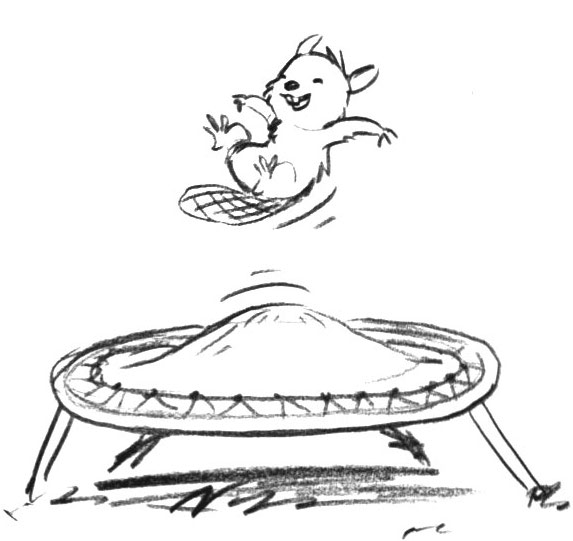
\includegraphics[width=2in]{Trampoline_Beaver_by_FancyFerret.jpg}\hspace{2mm}\footnote{\url{http://fancyferret.deviantart.com/art/Trampoline-Beaver-166211545}, CC BY-NC 3.0 license, Josef Ek.}}
\author{Jean-Luc B\'echennec, IRCCyN}
\date{June 4 \& 5, 2015}                                           % Activate to display a given date or no date

\begin{document}

\maketitle

{\bf Note:} All the software and documents are stored at \url{http://www.irccyn.ec-nantes.fr/~bechenne/trampoline}

\section{Goal}

The goal of this training is to become familiar with OSEK/VDX applications development process and with Trampoline. Trampoline is a Free Software implementation of the OSEK/VDX specification. Trampoline includes an OIL compiler which allows, starting from an OIL description, to generate OS level data structures of the application. In addition to the OIL description, the developer must provide the C sources of tasks and ISRs of the application. Trampoline runs on many  hardware platforms and we will use it on the Cortex-M4 STM32F4 Discovery board. If you have not installed Trampoline yet, get the Trampoline Package and read the install document.

The source code is located in the \unixcl{labs/labs_stm32F4_discovery} directory.

\section{The board}

We are going to use a demo board made by ST, the STM32F4 Discovery, with a Cortex M4 STM32F407 micro-controller. Here is a picture of the demo board:

\begin{center}
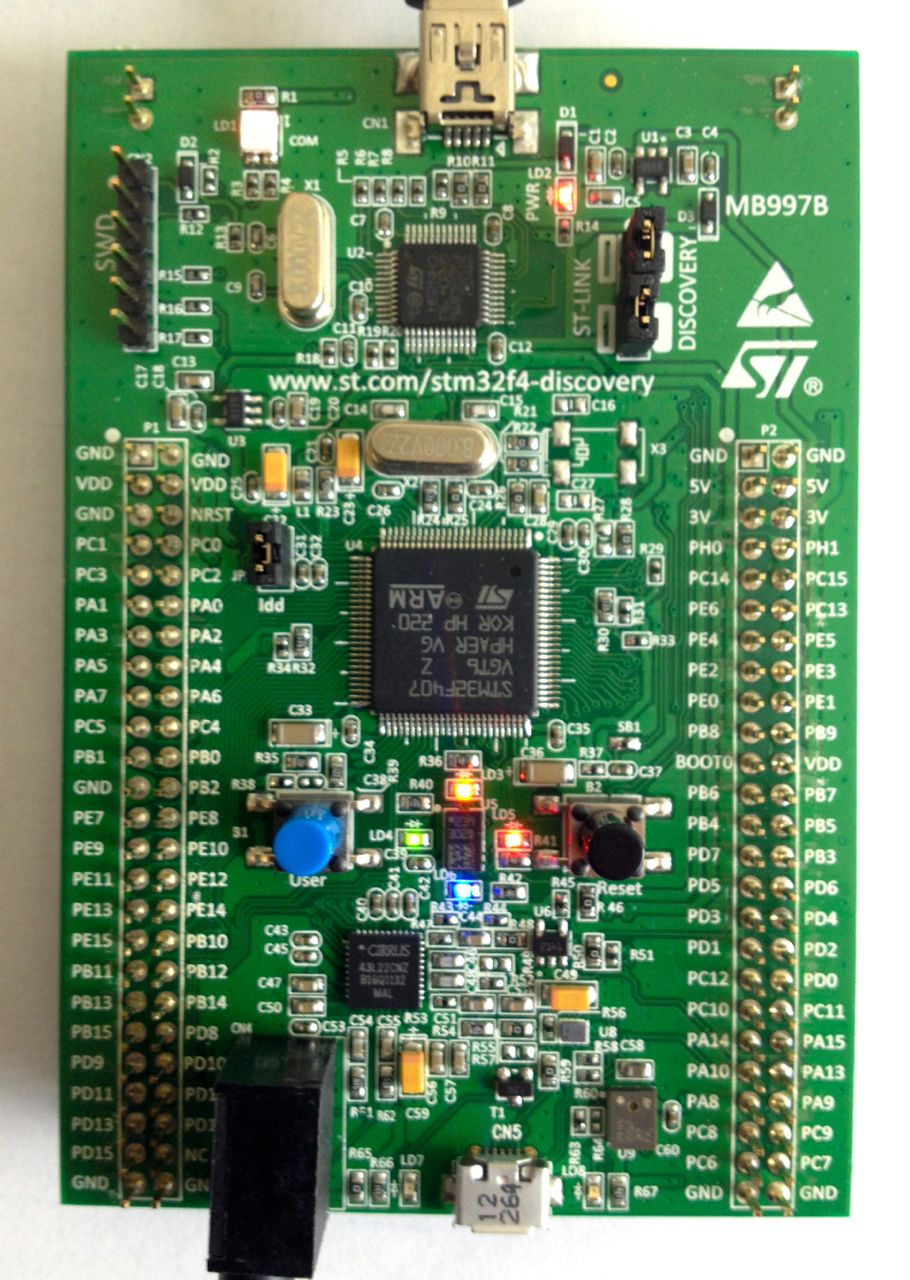
\includegraphics[width=.8\textwidth]{discovery.jpg} 
\end{center}

There are 4 LEDs located below the micro-controller. \LEDorange\ is the \textcolor{orange}{orange} one,  \LEDgreen\  is the \textcolor{LimeGreen}{green} one, \LEDred\ is the \textcolor{red}{red} one and \LEDblue\ is the \textcolor{blue}{blue} one. 

On the left, there is a \fcolorbox{blue}{LightSkyBlue}{blue button} labelled \texttt{User} that can be used for user interaction. On the right, there is a \fcolorbox{black}{black!20}{black button} which is the reset button.

The LEDs and the blue button are connected to the GPIO of the micro-controller. The GPIO is initialized with the LEDs as output and the button as input. The input corresponding to the button may be configured as an external interrupt line. The initialization is done by calling the \lstinline{initBoard} function. The argument of this function may be \lstinline{BUTTON_NOIT} to configure the corresponding GPIO input as a normal input or  \lstinline{BUTTON_IT} to configure the input as an external interrupt line. In summary \lstinline{initBoard(BUTTON_NOIT);} or \lstinline{initBoard(BUTTON_IT);} should be put in the \lstinline{main} function before starting Trampoline as shown below:

\begin{lstlisting}
FUNC(int, OS_APPL_CODE) main(void)
{
  initBoard(BUTTON_NOIT);
  StartOS(OSDEFAULTAPPMODE);
  return 0;
}
\end{lstlisting}

For the labs, functions are provided to switch on, switch off and toggle the LEDs. The unique argument is the LED identifier and should be \LEDorange, \LEDgreen, \LEDred\, \LEDblue\ or \textcolor{orange}{ORANGE},  \textcolor{LimeGreen}{GREEN}, \textcolor{red}{RED}, \textcolor{blue}{BLUE}:

\unixcl{void ledOn(<led>)} turns on LED \lstinline{<led>}.\\
\unixcl{void ledOff(<led>)} turns off LED \lstinline{<led>}.\\
\unixcl{void ledToggle(<led>)} toggles LED \lstinline{<led>}.

A function gives the state of the  \texttt{User} blue button. It returns \lstinline{BUTTON_PRESSED} if the button is pressed and \lstinline{BUTTON_RELEASED} if not.

\unixcl{ButtonState readButton();} returns the state of the \texttt{User} blue button. 

At last a function called \lstinline{delay} waits for an amount of time expressed in milliseconds.

\unixcl{void delay(<howManyMs>);} waits \lstinline{<howManyMs>} ms. 

Will will use this function to slow down the application.

\subsection{A word about memory sections}

AUTOSAR defines a way to put objects: constants, variables and functions in memory sections in a portable way\footnote{memory section declaration is not part of the C standard}. For that, a set of macro are used along with a generated file : MemMap.h. Functions should be declared with the \lstinline{FUNC} macro, variables with the \lstinline{VAR} macro, constants with the \lstinline{CONST} macro and pointers to variables, pointers to constant, constant pointers to variable and constant pointers to constant with \lstinline{P2VAR}, \lstinline{P2CONST}, \lstinline{CONSTP2VAR} and \lstinline{CONSTP2CONST} respectively. Sections are opened and close with a macro definition and the inclusion of the \lstinline{tpl_memmap.h} file. For instance:

\begin{lstlisting}
#define APP_Task_my_periodic_task_START_SEC_VAR_32BIT
#include "tpl_memmap.h"
VAR(int, AUTOMATIC) period;
VAR(int, AUTOMATIC) occurence;
#define APP_Task_my_periodic_task_STOP_SEC_VAR_32BIT
#include "tpl_memmap.h"
\end{lstlisting}

defines variables \lstinline{period} and \lstinline{occurence} in the variables section of task \lstinline{my_periodic_task}.

\begin{lstlisting}
#define APP_Task_my_periodic_task_START_SEC_CODE
#include "tpl_memmap.h"
TASK(my_periodic_task)
{
  ...
  TerminateTask();
}
#define APP_Task_my_periodic_task_STOP_SEC_CODE
#include "tpl_memmap.h"
\end{lstlisting}

defines the task \lstinline{my_periodic_task} in the code section of task \lstinline{my_periodic_task}. \lstinline{goil} generates the sections for tasks according to the description.

\section{Basic tasks}

Go into the lab1 directory. There are 2 files:

\begin{description}
\item[lab1.oil] the OIL description of the lab1 application;
\item[lab1.c] the C source for the lab1 task.
\end{description}

Edit the lab1.oil and look at the \texttt{TRAMPOLINE_BASE_PATH} attribute (in OS $>$ BUILD attribute).  \texttt{TRAMPOLINE_BASE_PATH} is set to \texttt{"../../.."}. If you move around the lab1 directory you will have to update this attribute.

lab1 is a very simple application with only 1 task called \lstinline{a_task}. \lstinline{a_task} starts automatically (\texttt{AUTOSTART = TRUE} in the OIL file). Look at the OIL file and the C source file.

To compile this application, go into the lab1 directory and type:\\
\unixcl{goil -t=thumb2/cortex-m4/STM32F4-Discovery lab1.oil}

%Goil templates are located in \texttt{trampoline/goilv2/templates}.
\texttt{goil} is the OIL compiler. It parses the OIL file and produces a set of C files. The \texttt{-t} option gives the target system. \texttt{thumb2} is the instruction set of the target, \texttt{cortex-m4} is the micro-controller core and \texttt{STM32F4-Discovery} is the board.\\\texttt{thumb2/cortex-m4/STM32F4-Discovery} is a path inside the \texttt{machines} directory and in the \texttt{templates} directory. The OIL file gives the names of the C source files (with \texttt{APP_SRC} and the name of the executable file (with \texttt{APP_NAME}).

This generate a Makefile for the application too. It has to be done only once. If you change something in the OIL file or in your C file, you do not need to rerun the goil compiler by hand because make will run it when needed. Then type:

\unixcl{make}

The application and Trampoline OS are compiled and linked together. To load the application on the target, type:

\unixcl{make burn}

The application may or may not start :-). Press the reset button if it does not start.

In this application, there is only one task called \lstinline{a_task} which switches \LEDorange\ on.

\begin{lstlisting}
TASK(a_task)
{
  ledOn(LED3);
  TerminateTask();
}
\end{lstlisting}

\section{OS system calls and task launching}

\subsection{Task activation and scheduling}


The \texttt{ActivateTask()} system call allows to activate another task of the application.

Go into the \texttt{lab2} directory.

In \texttt{lab2.oil} and \texttt{lab2.c}, 2 tasks have been added: \texttt{task_0} (priority 1) and \texttt{task_1} (priority 8). \texttt{task_0} toggles \LEDgreen\ on and \texttt{task_1} toggles \LEDred\ on. Task \texttt{a_task} activates \texttt{task_0} and \texttt{task_1}. All statements are separated by a busy-wait loop on the button so that by pressing the button we can control the execution. Examine the OIL and the C files.

Compile and execute. Why does \texttt{task_1} execute before \texttt{task_0} whereas it has been activated after?

\subsection{Task chaining}

The \texttt{ChainTask()} system call allows to chain the execution of a task to another one. This is roughly the same thing as calling ActivateTask and TerminateTask at the same time.

Replace the call to \texttt{TerminateTask} by a \texttt{ChainTask(task_1)} at the end of task \texttt{a_task}. What is happening?

Chain to \texttt{task_0} instead of \texttt{task_1}. What is happening?

Test the error code returned by \texttt{ChainTask} and correct your program to
handle the error. \texttt{ChainTask} may return the following codes:

\begin{description}
\item[E_OS_ID] the target task does not exist;
\item[E_OS_RESOURCE] the calling task holds a resource;
\item[E_OS_CALLEVEL] not called from a task;
\item[E_OS_LIMIT] too many activations of the target task.
\end{description}

\subsection{Pre-task and Post-task hooks}

Hook routines are used to insert application functions inside the kernel. Hook routines are called by the kernel when a particular event happens. The Pre-task hook is called when a task goes into the running state. The Post-task hook is called when a task leaves the running state. Hooks are useful for debugging purpose.

There are two boolean attributes in the OS object of the OIL to use Pre-task and Post-task hooks:

\begin{lstlisting}[language=OIL]
  OS config {
    STATUS = EXTENDED;
    PRETASKHOOK = TRUE;
    POSTTASKHOOK = TRUE;
    
  ...
\end{lstlisting}

When these hooks are used, the user have to write a hook functions:

\begin{lstlisting}
FUNC(void, OS_CODE) PreTaskHook()
{
  ...
}
\end{lstlisting}

for the pre-task hook and

\begin{lstlisting}
FUNC(void, OS_CODE) PostTaskHook()
{
  ...
}
\end{lstlisting}


Go into the \texttt{lab3} directory and play with the application which is in it. It is the same application as in \lstinline{lab2} with the use of \lstinline{delay} instead of busy-wait for the blue button. Pre and post task hooks are used to switch a led corresponding to the running task on.

\subsection{Extended tasks and synchronization using events}

Go into the \lstinline{lab4} directory.

This application has 2 tasks : \lstinline{a_task} which is an extended task and \lstinline{task_0} which is a basic task. Unlike a basic task, an extended task may wait for an event. A task is extended because it has at least one event declared in the OIL file.

Look at the OIL file and at the C file. Task \lstinline{a_task} activates task \lstinline{task_0} then goes into an infinite loop where it waits for event \lstinline{ev_0} and activate task \lstinline{task_0} again. When \lstinline{a_task} runs, \LEDorange\ is switched on. When \lstinline{task_0} runs, \LEDgreen\ is switched on. The application should run infinitely. 

\begin{ex}
Draw the Gantt diagram of the execution.
\end{ex}

\begin{ex}
However The application stops. What is happening ? Correct the OIL file to have a proper behavior.
\end{ex}

For the following application, we will use \lstinline{WaitEvent}, \lstinline{GetEvent} and \lstinline{ClearEvent}.
\begin{ex}
Extend the previous application by adding 1 task: \texttt{task_1} (priority 1) and 1 event \texttt{ev_1}. \texttt{a_task} activates \texttt{task_0} and \texttt{task_1} and waits for one of the events. When one of the events is set, \texttt{a_task} activates the corresponding task again.
\end{ex}

\section{Alarms, periodic tasks and ISR2}

\subsection{First application, basic use of alarms}

Go into the lab5 directory.

Alarms are periodic activities. They are used to build periodic tasks. Alarms may activate a task or set an event. The application in the lab5 directory is a simple one that blinks the \LEDblue\ with a 500ms period. The \lstinline{SysTick} is every 1ms. So the period of the alarm is 250ms. Examine the \lstinline{lab5.oil} file and the \lstinline{lab5.c} file. The underlying counter \lstinline{SystemCounter} have a \lstinline{TICKSPERBASE} attribute. This attribute is the number of \lstinline{SysTick} needed to increment the counter by one. By default it is set to 1. Pre and Post tasks hooks are used. Add a \lstinline{delay(50);} juste after \lstinline{ledToggle(BLUE);} in order to see the execution of the task.

\begin{ex}
Increase the \lstinline{TICKSPERBASE} to 25 and change the \lstinline{ALARMTIME} and \lstinline{CYCLETIME} of the alarm \lstinline{blink_blink} to keep the same period.
\end{ex}

\begin{ex}
Program an application using 2 periodic tasks, \lstinline{t1} and \lstinline{t2}. \lstinline{t1} switches \LEDblue\ on and \lstinline{t2} switches  \LEDblue\ off. Both tasks have the same period (1s) but have an offset so that  \LEDblue\ is on during 150ms.
\end{ex}

\subsection{Second application, starting and stopping alarms}

Go into the lab6 directory.

This application reads the \BB\ using a periodic task that is activated every 50ms. If the button is pressed, the \LEDblue\ is toggled.

Using services \lstinline{GetAlarm}, \lstinline{SetRelAlarm} and \lstinline{CancelAlarm}, build an application with the following requirements:
\begin{itemize}
\item Alarm \lstinline{blink_blink} activates task \lstinline{blink}. This alarm is not an \lstinline{AUTOSTART} one.
\item Task \lstinline{blink} toggles \LEDgreen.
\item If the button is pressed and alarm \lstinline{blink_blink} is not yet started, start the alarm with a period of 100ms.
\item If the button is pressed and alarm \lstinline{blink_blink} is started, cancel the alarm.
\end{itemize}

\subsection{Third application}

Requirements change. Now blinking needs an Init code
(runs once when the alarm is started) and a Final code (runs once when the alarm is stopped).
This corresponds to the following diagram:

\begin{center}
\begin{adjustbox}{width=14cm,keepaspectratio}
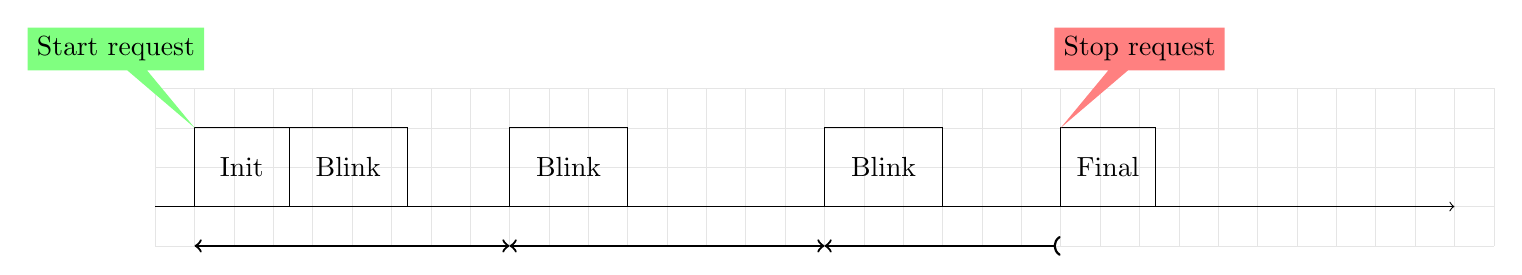
\begin{tikzpicture}
\draw[step=.5cm,gray!20,very thin] (-0.5, -0.5) grid (16.5,1.5);
\draw [->] (-0.5,0) -- (16,0);
\draw (0,0) rectangle (1.2,1);
\node at (0.6,0.5) {Init};
\draw (1.2,0) rectangle (2.7,1);
\node at (1.95,0.5) {Blink};
\draw (4,0) rectangle (5.5,1);
\node at (4.75,0.5) {Blink};
\draw (8,0) rectangle (9.5,1);
\node at (8.75,0.5) {Blink};
\foreach \x in {0, 4}
  \draw [xshift=\x cm,thick,<->] (0,-0.5) -- (4,-0.5); 
\draw [xshift=8 cm,thick,<-(] (0,-0.5) -- (3,-0.5); 
\draw [xshift=11cm] (0,0) rectangle (1.2,1);
\node [xshift=11cm] at (0.6,0.5) {Final};
\node [rectangle callout, fill=green!50, callout absolute pointer={(0,1)}] at (-1,2) {Start request};
\node [rectangle callout, fill=red!50, callout absolute pointer={(11,1)}] at (12,2) {Stop request};
\end{tikzpicture}
\end{adjustbox}
\end{center}


\begin{ex}
Modify the application to take the new requirements into account. Use 3 basic tasks. Init and Final blink their own LED once (use delay to see the execution).
\end{ex}

\begin{ex}
Same question but with only one extended task.
\end{ex}

\subsection{Chase}

Program a chase\footnote{chenillard in French} with a 0.5s period. To do it, use 4 periodic tasks. Each periodic task manages a LED. The chase effect is done by using alarms with a time shift between them.

When the \BB\ is pressed, the chase direction changes.

\subsection{Using an ISR2}

Instead of polling the \BB\, we are going to use and interrupt to trigger an ISR2. Go into the lab7 directory. Use the application as a starting point to replace button polling by ISR2 in the chase application.

\section{Shared object access protection}

\subsection{Goal}

To show resources usage, we will use a bad program that allows to corrupt a shared global variable which is not protected against concurrent writes. We will see different ways to prevent this wrong behavior by using resources (standard and internal) or other solutions (preemption and priority).

\subsection{Application requirements}

The application has 3 tasks and 2 \textbf{volatile} global variables: \texttt{val} and \texttt{activationCount} as shown in figure \ref{fig:appdiag}:

\def\alarm#1#2{
  \node[alarm](#1) [#2] {};
  \coordinate (a) at ($(#1.north)$);
  \coordinate (b) at ($(#1.north east)$);
  \coordinate (c) at ($(#1.north west)$);
  \coordinate (d) at ($(#1)$);
  \draw[thick] ($(a)+(-0.1,0)$) rectangle ($(a)+(0.1,0.1)$);
  \draw[rotate=-45,thick] ($(b)+(-0.05,0)$) rectangle ($(b)+(0.05,0.1)$);
  \draw[rotate=45,thick] ($(c)+(-0.05,0)$) rectangle ($(c)+(0.05,0.1)$);
  \draw ($(d)+(0.3,0)$) -- (d) -- ($(d)+(0,0.3)$);
  \node [font=\scriptsize,below=0.5mm of #1] {{\em Alarm}}
}

\def\sharedvar#1#2#3{
  \node (#1) [#2] {#1};
  \coordinate (a) at ($(#1.north #3) + (0,0.2)$);
  \coordinate (b) at ($(#1.south #3) + (0,-0.2)$);
  \draw[ultra thick] (a) -- (b);
  \draw ($(a)+(-0.1,0)$) -- ($(a)+(0.1,0)$); 
  \draw ($(b)+(-0.1,0)$) -- ($(b)+(0.1,0)$) 
}

\def\varrect#1{
  \draw ($(#1.south west)$) rectangle ($(#1.north east)$)
}

\begin{figure}[htb] %  figure placement: here, top, bottom, or page
   \centering
   \begin{tikzpicture}[
   task/.style={draw,very thick,fill=white,drop shadow={opacity=0.25},text width=2.5cm, text centered, minimum height=1.5cm},
   alarm/.style={draw,thick,circle,fill=white,drop shadow={opacity=0.25},text width=.5cm}
   ]
   \node[task](periodicTask) at (0,0) {periodicTask};
   \node[task](bgTask) [above=of periodicTask] {bgTask};
   \node[task](displayTask) [above=of bgTask] {displayTask};
   \alarm{activateDisplay}{left=20mm of displayTask};
   \alarm{activatePeriodic}{left=20mm of periodicTask};
   \sharedvar{val}{left=of bgTask}{east};
   \sharedvar{activationCount}{right=of periodicTask}{west};
   \sharedvar{LED4}{right=of displayTask}{west};
   \sharedvar{LED5}{above right=of displayTask}{west};
   \varrect{LED4};
   \varrect{LED5};
   \draw [thick,<->] (val.east) -- (bgTask.west);
   \draw [thick,->] (val.north east) -- ++(5mm,0) |- ($(displayTask.south west) + (0,2mm)$);
   \draw [thick,<->] (val.south east) -- ++(5mm,0) |- ($(periodicTask.north west) + (0,-2mm)$);

   \draw [thick,->] (activateDisplay.east) -- ++(5mm,0) -- ++(0,1.5mm) -- ++(3mm,-3mm) -- ++ (0mm,1.5mm) -- (displayTask);
   \node at ($(activateDisplay.east) + (6.5mm,-3mm)$) {1s};
   \node[font=\scriptsize] at ($(activateDisplay.east) + (9mm,3mm)$) {{\em ActivateTask}};
   \draw [thick,->] (activatePeriodic.east) -- ++(5mm,0) -- ++(0,1.5mm) -- ++(3mm,-3mm) -- ++ (0mm,1.5mm) -- (periodicTask);
   \node at ($(activatePeriodic.east) + (6.5mm,-3mm)$) {100ms};
   \node[font=\scriptsize] at ($(activatePeriodic.east) + (9mm,3mm)$) {{\em ActivateTask}};
   \draw [thick,<->] (activationCount.west) -- (periodicTask);
   \draw [thick,->] (activationCount.north west) -- ++(-5mm,0) |- ($(displayTask.south east) + (0,2mm)$);
   \draw [thick,->] (displayTask) -- (LED4);
   \draw [thick,->] (displayTask.north) |- (LED5);
   \end{tikzpicture} 
   \caption{Application diagram}
   \label{fig:appdiag}
\end{figure}

\begin{itemize}
\item a background task called \texttt{bgTask}, active at start (\texttt{AUTOSTART = TRUE}) and that never ends. In an infinite loop this task increments then decrements the global variable \texttt{val}. This task has a priority equal to 1.

\item a periodic task called \texttt{periodicTask}, priority 10, that runs every 100ms. This periodic task increments the global variable \texttt{activationCount} which is initialized to 0 at start. Then if \texttt{activationCount} is odd, \texttt{val} is incremented, otherwise it is decremented.

\item a periodic task \texttt{displayTask}, priority 20, that runs every second. If \texttt{val} is inside interval $[-1;2]$, \LEDgreen\ is switched on and \LEDred\ is switched off. Otherwise, \LEDred\ is switched on and \LEDgreen\ is switched off.
\end{itemize}

Describe the application in OIL and program it in C.

\begin{ex}
Does the behavior correspond to what you expect ? Why ?
\end{ex}

\subsection{Global variable protection}

\begin{ex}
Update the OIL file and the C program to protect the access to the global variable \texttt{val}. Use a resource to do it.
\end{ex}

The resource priority is automatically computed by goil according to the priorities of the tasks which use it.

\begin{ex}
What priority will be given to the resource ?
\end{ex}

The OIL compiler (goil) generates many files in the directory bearing the same name
as the oil file (less the .oil suffix). Among them 3 are interesting:
\begin{itemize}
\item \texttt{tpl_app_define.h}
\item \texttt{tpl_app_config.h}
\item \texttt{tpl_app_config.c}
\end{itemize}

The file \texttt{tpl_app_config.c} contains the tasks' descriptors as long as all other data structures. These structures are commented.

\begin{ex}
For each task, find the priority computed by goil and the identifier. Is is the same as defined in the OIL file? if not is it a problem?
\end{ex}

\begin{ex}
What is the priority of the resource? Is it compliant with the PCP rule?
\end{ex}

\subsection{Protection with an internal resource}

An internal resource is automatically taken when the task gets the CPU. Replace the standard resource by an internal resource in the OIL file. Remove the \texttt{GetResource} and \texttt{ReleaseResource} in the C file.

\begin{ex}
What happens ? Why ?
\end{ex}

Modify the task \texttt{bgTask}: instead of infinite loop, use a \texttt{ChainTask} to the \texttt{bgTask} (ie: the task chains to itself).

\begin{ex}
What happens ? Explain.
\end{ex}

\section{Adding a service into Trampoline}

In this part we are going to see how to add semaphore services into Trampoline. We want two services : \lstinline{SemWait} to lock a semaphore and \lstinline{SemPost} to unlock a semaphore.

\begin{figure}[htbp] %  figure placement: here, top, bottom, or page
   \centering
   \includegraphics[width=3in]{SemaphoreSEM.pdf} 
   \caption{A semaphore object}
   \label{fig:example}
\end{figure}

\subsection{Adding a semaphore object}

Let's start with the data. 

\paragraph{The first thing} to do is to provide an object type for semaphores in C. We need a \lstinline{struct} with four members. \lstinline{token} is the current number of token available. \lstinline{size} is the number of tasks waiting in \lstinline{waiting_tasks}. \lstinline{index} is write index in \lstinline{waiting_tasks}. \lstinline{waiting_tasks} is a ring buffer to store the tasks waiting for the semaphore.

\begin{lstlisting}
typedef struct {
  uint32      token;
  uint32      size;
  unit32      index;
  tpl_task_id waiting_tasks[TASK_COUNT];
} tpl_semaphore;
\end{lstlisting}

\lstinline{TASK_COUNT} is computed by goil and is equal to the number of tasks in the application. 

\paragraph{The second thing} is to provide an object type for semaphores in the OIL description. This is done in the \lstinline{IMPLEMENTATION} part of the OIL description. Normally the OIL standard does not allow to create new object types. This has been relaxed in goil.

\begin{lstlisting}
SEMAPHORE [] {
  UINT32 TOKEN;
};
\end{lstlisting}

This declares a new object type : \lstinline{SEMAPHORE} with an \lstinline{UINT32} attribute, \lstinline{TOKEN}. The \lstinline{[]} means multiple instances of semaphore can be used.
Now, semaphores can be declared in the OIL file:

\begin{lstlisting}
SEMAPHORE sem1 { TOKEN = 3; };
SEMAPHORE sem2 { TOKEN = 1; };
\end{lstlisting}

\paragraph{The third thing} is to write a template that will generate C source code with a \lstinline{tpl_semaphore} instance for each \lstinline{SEMAPHORE} object in the OIL file. To do that, we have to provide a template directory hierarchy as in \lstinline{goilv2/templates}. This hierarchy is put in the directory where the application source files are.

Since we generate code, the hierarchy is \lstinline{goilv2/code}. Our code  will be embedded in the \lstinline{tpl_app_config.c} and \lstinline{tpl_app_define.h}.

The templates are \lstinline{custom_app_config.goilTemplate} and \lstinline{custom_app_define.goilTemplate} respectively.

In the first one we have to:
\begin{enumerate}
\item generate semaphore object identifiers. A semaphore object identifier has the \lstinline{SemType} type;
\item generate semaphore objects. A semaphore object has the \lstinline{tpl_semaphore} type;
\item generate a semaphore table indexed by semaphore object identifiers. Each element of this table is a pointer to the corresponding semaphore object.
\end{enumerate}

\subsection{Semaphore services}

Services are described in configuration OIL files. To add a service, we must provide a description of the service. This can be done in the OIL file of the application as follow :

\begin{lstlisting}
APICONFIG semaphore {
  ID_PREFIX = OS;
  FILE = "tpl_os_semaphore_kernel";
  HEADER = "tpl_os_semaphore";
  SYSCALL SemWait {
    KERNEL = tpl_sem_wait_service;
    RETURN_TYPE = StatusType;
    ARGUMENT sem_id { KIND = CONST; TYPE = SemType; };
  };
  SYSCALL SemPost {
    KERNEL = tpl_sem_post_service;
    RETURN_TYPE = StatusType;
    ARGUMENT sem_id { KIND = CONST; TYPE = SemType; };
  };
};
\end{lstlisting}

\lstinline{APICONFIG} is the root object to define a set of services related to a new object. Here we define an \lstinline{APICONFIG} for semaphores. goil generates identifiers for services. Identifiers are prefixed by a section name. For instance, operating system services are prefixed by OS and communication services are prefixed by COM. Here we choose to use the OS prefix: \lstinline{ID_PREFIX = OS;}

The \lstinline{FILE} attribute allows to list the files where the C kernel function are defined. As many files as needed may be listed. The \lstinline{HEADER} attribute allows to list the files where the datatypes and constants are declared. As many files as needed may be listed. 

The \lstinline{SYSCALL} attribute is used to define a service. The name, here \lstinline{SemWait} and \lstinline{SemPost}, is the service name as seen by the application. \lstinline{KERNEL} is the corresponding kernel function. \lstinline{RETURN_TYPE} is the type of variable returned by the service and \lstinline{ARGUMENT} is the name, type and kind of argument. As many arguments as needed may be listed (almost).

The corresponding C source code must be provided in files \lstinline{tpl_os_semaphore_kernel.h}, \lstinline{tpl_os_semaphore_kernel.c} and \lstinline{tpl_os_semaphore.h}.

At last, the template \lstinline{api.goilTemplate} is modified to add the following template code:
\begin{lstlisting}
if exists SEMAPHORE then
  if [SEMAPHORE length] > 0 then
    let APIUSED += APIMAP["semaphore"]
  end if
end if
\end{lstlisting}

\end{document}  